% !TEX root = mgcv.tex

\begin{block}{Smoothers}
  Using the \texttt{bs=} argument in \texttt{s()}, \texttt{te()}, etc. Further details can be found in \texttt{?smooth.construct.*.smooth.spec}\br

  \begin{subblock}{Univariate only smoothers}
    \begin{columns}
      \begin{column}{0.5\linewidth}
        Cubic regression splines \texttt{cr}\br
        Cubic regression splines with shrinkage \texttt{cs}\br
        B-splines \texttt{bs}\br
        P-splines \texttt{ps}\br
      \end{column}
      \begin{column}{0.5\linewidth}
        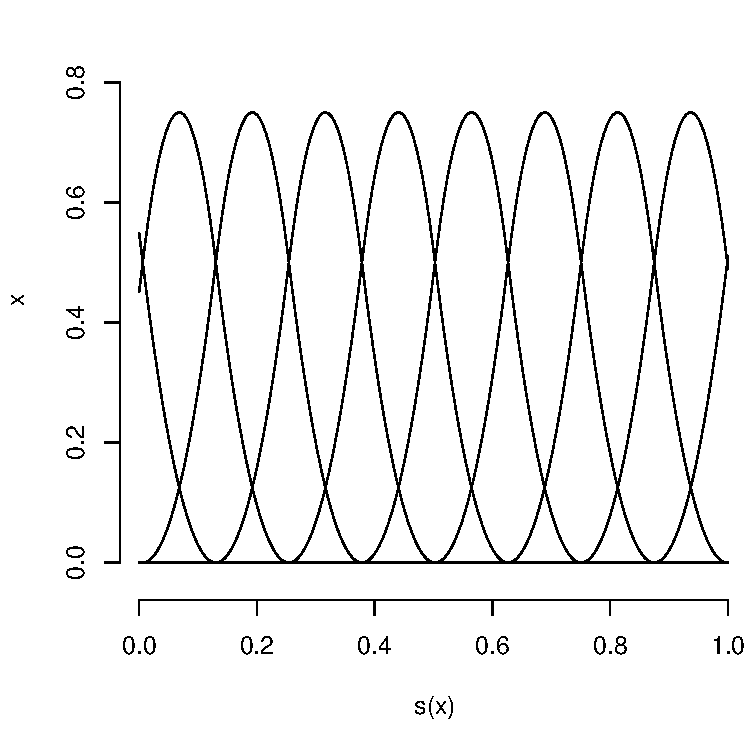
\includegraphics[width=0.2\textwidth]{bsplines.pdf}
      \end{column}
    \end{columns}
  \end{subblock}

  \vskip-2ex
  \begin{columns}[t]\hfill\hfill\hfill
    \begin{column}{.48\linewidth}
      \begin{subblock}{Special smoothers}
Cyclic cubic splines \texttt{cc}\br
Adaptive smoothers \texttt{ad}\br
Factor-smooth interactions \texttt{sz}\br
Random factor-smooth interactions \texttt{fs}
      \end{subblock}
    \end{column}\hfill
    \begin{column}{.48\linewidth}
      \begin{subblock}{Smoothers in $\geq1$ dimension}
Thin plate regression splines \texttt{tp}\br
Thin plate regression splines within shrinkage \texttt{ts}\br
Duchon splines \texttt{ds}\br
Random effects \texttt{re}\br
Markov random fields \texttt{mrf}\br
Gaussian process smooths \texttt{gp}
      \end{subblock}
      \begin{subblock}{Smoothers in 2 dimensions}
Splines on the sphere \texttt{sos}\br
Soap film smoothing \texttt{so} (\texttt{sw} and \texttt{sf})
      \end{subblock}
      \end{column}\hfill\hfill\hfill
    \end{columns}


\end{block}
